% !TEX TS-program = pdflatex
% !TEX encoding = UTF-8 Unicode

% This is a simple template for a LaTeX document using the "article" class.
% See "book", "report", "letter" for other types of document.

\documentclass[11pt]{article} % use larger type; default would be 10pt

\usepackage[utf8]{inputenc} % set input encoding (not needed with XeLaTeX)

%%% Examples of Article customizations
% These packages are optional, depending whether you want the features they provide.
% See the LaTeX Companion or other references for full information.

%%% PAGE DIMENSIONS
\usepackage{geometry} % to change the page dimensions
\geometry{a4paper} % or letterpaper (US) or a5paper or....
% \geometry{margin=2in} % for example, change the margins to 2 inches all round
% \geometry{landscape} % set up the page for landscape
%   read geometry.pdf for detailed page layout information

\usepackage{graphicx} % support the \includegraphics command and options

% \usepackage[parfill]{parskip} % Activate to begin paragraphs with an empty line rather than an indent

%%% PACKAGES
\usepackage{booktabs} % for much better looking tables
\usepackage{array} % for better arrays (eg matrices) in maths
\usepackage{paralist} % very flexible & customisable lists (eg. enumerate/itemize, etc.)
\usepackage{verbatim} % adds environment for commenting out blocks of text & for better verbatim
\usepackage{subfig} % make it possible to include more than one captioned figure/table in a single float
% These packages are all incorporated in the memoir class to one degree or another...

%%% HEADERS & FOOTERS
\usepackage{fancyhdr} % This should be set AFTER setting up the page geometry
\pagestyle{fancy} % options: empty , plain , fancy
\renewcommand{\headrulewidth}{0pt} % customise the layout...
\lhead{}\chead{}\rhead{}
\lfoot{}\cfoot{\thepage}\rfoot{}

%%% SECTION TITLE APPEARANCE
\usepackage{sectsty}
\allsectionsfont{\sffamily\mdseries\upshape} % (See the fntguide.pdf for font help)
% (This matches ConTeXt defaults)

%%% ToC (table of contents) APPEARANCE
\usepackage[nottoc,notlof,notlot]{tocbibind} % Put the bibliography in the ToC
\usepackage[titles,subfigure]{tocloft} % Alter the style of the Table of Contents
\renewcommand{\cftsecfont}{\rmfamily\mdseries\upshape}
\renewcommand{\cftsecpagefont}{\rmfamily\mdseries\upshape} % No bold!

%%% END Article customizations

%%% The "real" document content comes below...

\title{\textbf{Air Quality in China: Explorations}}
\author{Shengqian Chen, Alex Dewey, Ruoying Jiang, Xingxing Tong}
%\date{} % Activate to display a given date or no date (if empty),
         % otherwise the current date is printed 

\begin{document}
\maketitle

\begin{abstract}
Air quality in China is a major issue.\cite{Moore14} In this report, we did some data science about it.
\end{abstract}

\section{Introduction}

\subsection{Air Pollution}

\begin{figure}[!ht]
  \centering
    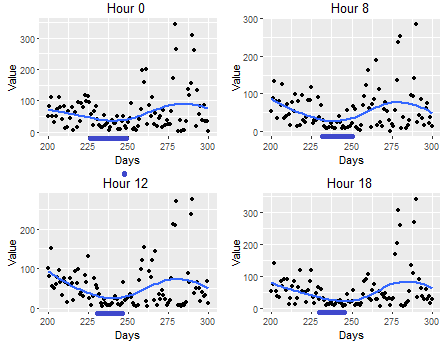
\includegraphics[width=0.6\textwidth]{ParadeBlueBeijing}
      \caption{\(\mathit{PM_{2.5}}\) \textit{during Beijing's Parade Blue}}
\end{figure}

A widely-circulated 2015 study from American
think tank Berkeley Earth estimated from available literature
as many as 1.2 to 2 million premature deaths a year from air pollution
in China alone. Particulate matter causes "premature death 
in people with heart and lung disease" per the EPA. 
These numbers are backed up by the World
Health Organization, the Lancet, and the IHME.

Former Health minister Chen Zhu published 
in the Lancet a conservative estimate of between
350,000 and 500,000 deaths a year. For comparison,
Dane, Iowa, Green, and Columbia counties (the 
Madison Metro statistical area) had a total
2010 population of 568,593.

Reliable, accessible data taken hourly.

Combined population of 5 cities' administrative areas is greater than
100 million people (some 1.5\% of the human population 
and 7\% of the population of China)

Air pollution is caused by human activity
such as industry, heating, and transportation
and cities are one obvious starting point
for China's efforts to improve air quality.

The data is measured in terms of \(PM_{2.5}\), which measures the 
total mass of fine particles in the atmosphere (micrograms
per cubic meter).

\subsection{Key Questions}

In August 2015, the Chinese government stopped much of its
industrial capacity and traffic for a 
WWII 70th anniversary celebration called "Parade Blue"\cite{Boren15}.

\(PM_{2.5}\) readings quickly dropped below 19.5 and averaged \(35 \mu g/m^3\)



Parade Blue demonstrated how sensitive particulate readings
are to short-term human activities (and reduction).

We're using hours 0, 8, 12, 18 in order to account
for the effect of the most important times of day
without overcomplicating things.

\section{Part 1 - Intuitive Exploration based on Visualization}



	Our dataset comes from the U.S. Department of State in the Embassy and Consulates of five major cities in China. Data is measured in terms of the total mass of particulate matter (particles with size 2.5 micrometers or less, which we denote as "PM 2.5"). The PM 2.5 data is hourly over the course of 2015, so there are 24 data points in each day for each of the five cities.

	The goal of this part is to explore the raw dataset based on visualization. We hope to get a big picture about the distribution of PM 2.5 among these five cities. Numerical analysis will be conducted in the next part.

	The nature of this dataset (and personal experience with air pollution) led us to a hypothesis that the pattern of P.M 2.5 varies from hour to hour. So we focused on four specific hours in the first stage of our exploration: We collected data at 12:00am, 8:00 am, 12:00 pm, and 6:00pm. 8:00 am and 6:00 pm are chosen since they are rush hours where we expect to see primary levels of transportation. 12:00am seems to be a solid baseline for low human activity and 12:00 pm is the midday, where we might expect lower transportation but higher industrial air pollution.

	Based on an informal comparison of these four hours, we made the assumption that the P.M 2.5 would be highly correlated with air pollution from traffic. We therefore expected to see relatively low P.M 2.5 at 12:00am and relatively high values at the 8:00 am and 6:00pm measurements.

	Below in Figure 1 is our PM 2.5 plot for all five cities at the four hours. Note that the graph is color-coded by site: SH means Shanghai, GZ is Guangzhou, CD indicates Chengdu, BJ is Beijing, and SY stands for Shenyang. 
	
	 \begin{figure}[!ht]
  \centering
    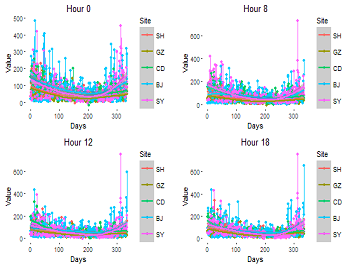
\includegraphics[width=0.6\textwidth]{Figure1-1}
      \caption{Each plot is the value of everyday \(PM_{2.5}\) at a particular time point (12:00 am, 8:00 am, 12:00 pm, and 6:00 pm) in 5 big cities in China (Shanghai, Guangzhou, Chengdu, Beijing, and Shenyang).
}
\end{figure}

	The density of points in Figure 1 from these five cities makes it hard to notice any pattern. So, as an exploration, we decided to focus the first 50 days of 2015 which gives us the following graph.
	

\begin{figure}[!ht]
  \centering
    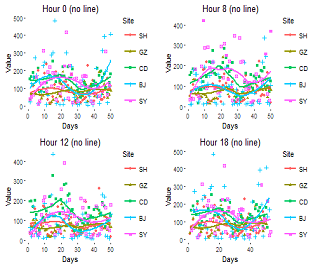
\includegraphics[width=0.6\textwidth]{Figure1-2}
      \caption{Four hours plots of 5 cities for the first 50 days}
\end{figure}

In order to make the pattern for each city more clearly we concentrate on Hour 0 and split cities apart. 

\begin{figure}[!ht]
  \centering
    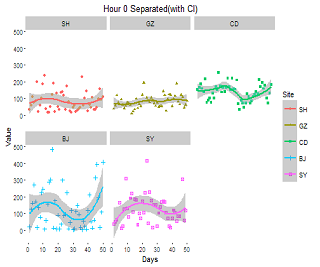
\includegraphics[width=0.6\textwidth]{Figure1-3}
      \caption{Hour 0 plots of 5 cities for the first 50 days}
\end{figure}

Figure 3 indicates that for the given hour and day period, Shanghai and Guangzhou maintain a very stable pattern. The P.M. 2.5 for Chengdu fluctuate a little bit. However, its pattern keeps stable in general. For Beijing and Shenyang, however, their P.M. 2.5 change violently for the first 50 days. Different latitudes and longitudes mays provide some information for us. Shanghai and Guangzhou are in the south of China. However, Beijing and Shenyang are in the north of China. 
	There is a very clear trend to go up for Beijing. It seems that the P.M. 2.5 for Beijing will be higher than other cities on average for the following days. This very intuitive analysis gives us a direction that we should focus our project on Beijing which is also the reason why we are trying to use the meteorological data to explain the P.M. 2.5 for Beijing in the second part of our project. 
	We also draw the plots for days 51-100 and days 101-150. These graphs also indicate that Beijing has very unique patterns than the rest of cities. So, in the next part we turns to regression model explaining Beijing’s P.M. 2.5 via meteorological data.
	
\begin{figure}[!ht]
  \centering
    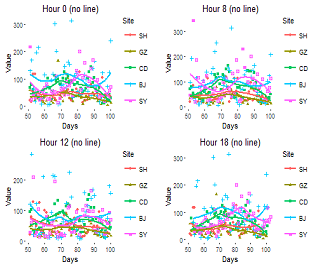
\includegraphics[width=0.6\textwidth]{Figure1-4}
      \caption{Four-hour plots of 5 cities for days 51-100}
\end{figure}

\begin{figure}[!ht]
  \centering
    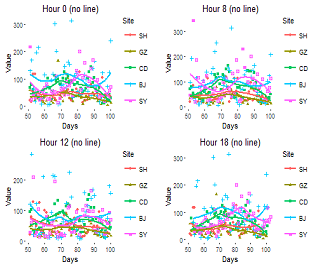
\includegraphics[width=0.6\textwidth]{Figure1-4}
      \caption{Four-hour plots of 5 cities for days 101-150}
\end{figure}

\newpage

\section{Part 2 - Regression fitting and Outlier Analysis}
\subsection{Regression of meteorological factors on daily average \(PM_{2.5}\)}

 \begin{quotation}
“Each country has different standards for \(PM_{2.5}\) mass concentration. To meet the standard for \(PM_{2.5}\), it is desirable to find the factors affecting \(PM_{2.5}\) concentration.”\cite{Chatani11}
 \end{quotation}
 
 Reports have argued that three factors can make an important effect on the \(PM_{2.5}\) mass concentration, which are domestic pollutants emission sources, external sources outside of the country, and the meteorological conditions
 
  \begin{quotation}
“As shown by previous studies, meteorological conditions can largely diffuse, dilute, and accumulate pollutants.”\cite{Pohjola02}
 \end{quotation}
 
  \begin{quotation}
“We find that daily variation in meteorology as described by the multiple linear regression can explain up to 50\% of \(PM_{2.5}\) variability with temperature, relative humidity (RH), precipitation, and circulation all being important predictors.”\cite{Tai10}
 \end{quotation}
 
 Thus, in the second part of our project, the key point is to figure out the relationship between meteorological variables and \(PM_{2.5}\) values in each day during 2015. 
Based on the analysis above about the hourly \(PM_{2.5}\) for 5 cities, Beijing is outstanding than other cities, presenting a higher level as a whole. Therefore, our first target for study is Beijing, the capital as well as political center of China. 
The meteorological data we obtained is from the weather underground website. In accordance with the daily average value of \(PM_{2.5}\), the meteorological factors being analyzed are the mean values of temperature, dew point, humidity, sea level pressure and wind speed in each day from January 1 to December 31 of 2015. Taken the lag effect into consideration, a lag factor is also included in our regression models, which is the average \(PM_{2.5}\) value one day before.
First we combine the meteorological data with the daily average\(PM_{2.5}\) data, then to fit our regression model. However, after drawing a graph of daily average \(PM_{2.5}\) during 2015, what we noticed is that it has a high beginning and end. In order to exclude the impacts of these extremely high values on our final model, it is obvious that we should focus only on days with normal \(PM_{2.5}\). According to the new air quality standards in China, we delete days that have average \(PM_{2.5}\) higher than 250\(\mu g/m^3\), which represents for a severe air pollution. And for 2015, Beijing has 18 days that the \(PM_{2.5}\) is larger than \(\mu g/m^3\).

 \begin{figure}[!ht]
  \centering
    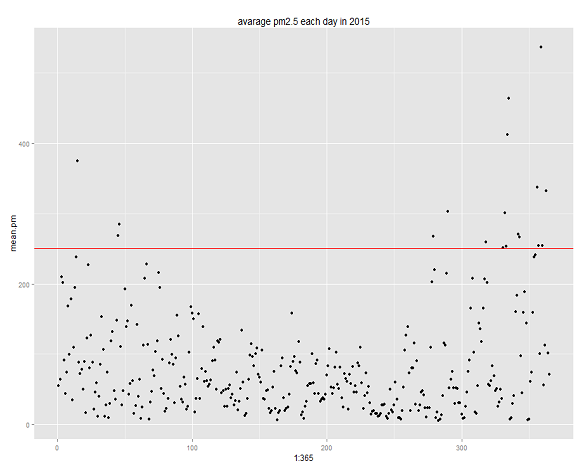
\includegraphics[width=0.6\textwidth]{Figure2-1}
      \caption{Daily average of \(PM_{2.5}\) measurements in Beijing for each day of 2015. The red line is at the value 250 \(\mu g / m^3\). We delete points above the red line in our model fitting.}
\end{figure}
 
 
 Next step, we start with the linear regression without interaction terms after filtering out days with \(PM_{2.5}\) larger than 250\(\mu g/m^3\). And for days \(PM_{2.5}>\mu g/m^3\), specific analysis is needed for further research. 
By summarizing the fitted model with all meteorological variables and one lag factor, we find out that only four variables are significant, which are the daily average values of temperature, sea level pressure, wind speed and the lag factor.
 
 \begin{table}
 \begin{tabular} {| r | r | r | r | r |}
 \hline
 \textbf{Variable} & 
\textbf{Estimated} & 
\textbf{Standard Error} & 
\textbf{t-value} \(\mathbf{t_0}\) & 
\(\mathbf{Pr(\vert t_0 \vert >t)}\) \\ \hline
\textbf{Intercept} & 1561.10 & 409.78 & 3.810 & 1.65 E-4 \\ \hline
\textbf{Lagged }\(\mathbf{PM_{2.5}}\) & 0.4485 & 0.0389 & 11.527 & \(<\)2 E-16 \\ \hline
\textbf{Temperature} & -1.20870 & 0.21537 & -5.612 & 4.14 E-8 \\ \hline
\textbf{Pressure (Sea Level)} & -46.729 & 13.278 & -3.519 & 4.91 E-4 \\ \hline
\textbf{Wind Speed} & -8.56 & 0.69 & -12.404 & \(<\)2 E-16 \\ \hline
 \end{tabular}
 \caption{Significant variables in the linear model.}
 \end{table}
 
Based on the table above, the estimated coefficients of mean temperature, mean sea level pressure and mean wind speed for each day are negative, which indicates the negative effects of these meteorological variables on the \(PM_{2.5}\) values. In contrast, the positive coefficient of lag(mean pm,1) suggests a positive relationship between \(PM_{2.5}\) and the lag factor.
Then we need to determine how well the model is. However, the adjusted R-squared is 0.5116, indicates the fitted model is not ideal. And in conjunction with the residual plot, which shows a strong pattern, we can say that a Non-linear regression is necessary in our future exploration. 

 


 \begin{figure}[!ht]
  \centering
    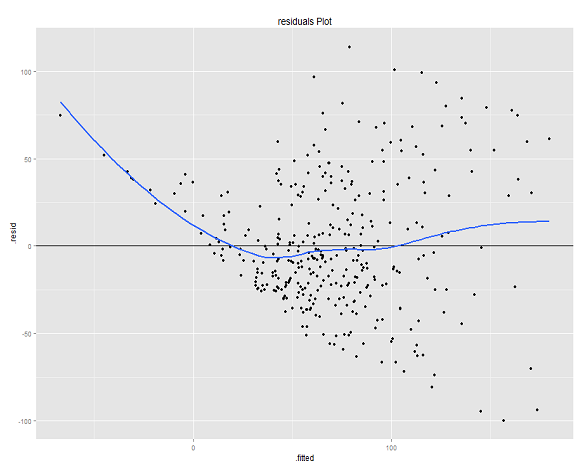
\includegraphics[width=0.6\textwidth]{Figure2-2}
      \caption{Residual plot of a linear regression on significant meteorogical factors versus daily average \(PM_{2.5}\) values}
\end{figure}

 \begin{figure}[!ht]
  \centering
    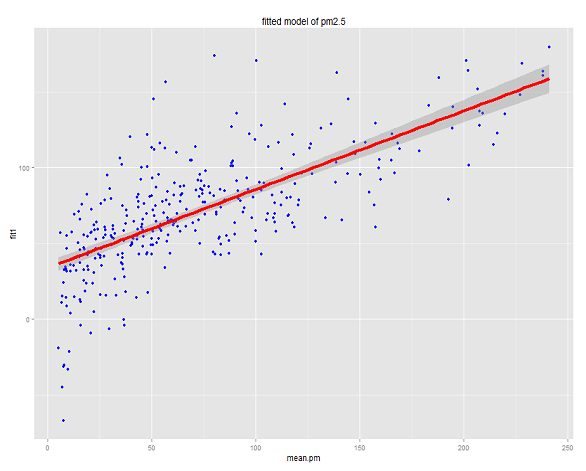
\includegraphics[width=0.6\textwidth]{Figure2-3}
      \caption{Fitted model plot of linear regression of daily average \(PM_{2.5}\) versus
      meterological factors, after deleting outliers.}
\end{figure}

Employ Box-Cox transformation to the fitted model, lambda is closer to 0, which indicates a log transformation is appropriate. So we refit the model by doing log transformation to the average \(PM_{2.5}\). According to the residual plot and larger adjusted R-square (0.5824), the new fitted model is better than the prior one, but still not good enough to explain the exact relationship.

 \begin{figure}[!ht]
  \centering
    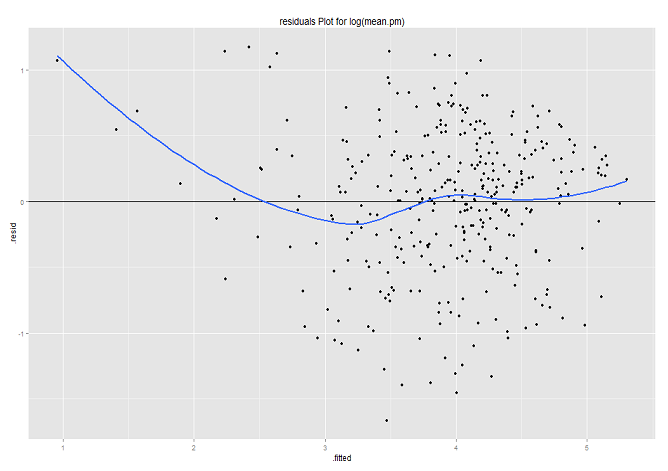
\includegraphics[width=0.6\textwidth]{Figure2-4}
      \caption{Residual plot of new fitted model after log transformation of daily average \(PM_{2.5}\). 18 outliers are still not included in the dataset.}
\end{figure}

\newpage

\subsection{Exploring outliers with \(PM_{2.5}\) > 250}

 \begin{figure}[!ht]
  \centering
    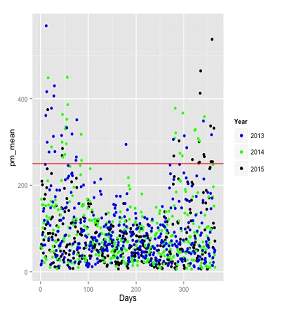
\includegraphics[width=0.6\textwidth]{Figure2-5}
      \caption{Daily averages for every day from 2013-2015--points from 2013 are displayed in blue, points from 2014 in green, and points from 2015 in black.}
\end{figure}

As we can see in the previous plot, the outliers of 2015 were concentrated in January, Feburary, October and December. These are the months when temperatures are relatively low within a year. Naturally, we want to see if this phenomenon is a pattern across 3 years. 

\begin{tabular}{| ccc | ccc | ccc |}
\hline
\multicolumn{3}{|c|}{2013} & 
\multicolumn{3}{|c|}{2014} &
\multicolumn{3}{|c|}{2015} \\ \hline
Month & Day & Mean PM 2.5 & 
Month & Day & Mean PM 2.5 &
Month & Day & Mean PM 2.5 \\ \hline
1 & 11 & 361.2 &1 & 16 & 448.4 &1 & 15 & 374.8 \\
1 & 12 & 568.6 &1 & 23 & 288.4 &2 & 14 & 268.5  \\
1 & 13 & 416.3 &2 & 14 & 299.7 &2 & 15 & 285  \\
1 & 14 & 299.5 &2 & 15 & 363.8 &10 & 6 & 267.7 \\
1 & 18 & 276.8 &2 & 16 & 264.8 &10 & 17 & 302.7  \\
1 & 23 & 378.1 &2 & 20 & 271 &11 & 14 & 259.3  \\
1 & 27 & 313 &2 & 21 & 330.4 &11 & 27 & 251.4  \\
1 & 28 & 406.4 &2 & 22 & 335.5 &11 & 28 & 300.5  \\
1 & 29 & 429.8 &2 & 23 & 296 &11 & 29 & 253.2 \\
1 & 30 & 277.9 &2 & 24 & 352.6 &11 & 30 & 412.8  \\ 
2 & 13 & 315 &2 & 25 & 449.8 &12 & 1 & 464.4  \\
2 & 24 & 332.9 &2 & 26 & 386.4 &12 & 8 & 270.9   \\
3 & 7 & 318.5&3 & 26 & 317.9 &12 & 9 & 266.2  \\
3 & 15 & 257.5 &3 & 27 & 257.4 &12 & 22 & 337   \\
3 & 16 & 265.2 &10 & 8 & 308.8&12 & 23 & 254.5  \\
3 & 17 & 351.3 &10  & 9 & 378 &12 & 25 & 537.2   \\
6 & 28 & 294.5 &10 & 10 & 321.1 &12 & 26 & 254.3  \\
10 & 5 & 306 &10  & 19 & 274 &12 & 29 & 331.9  \\
10  & 28 & 314.3 &10 & 25 & 267.8 &&& \\
11 & 2 & 286.8 &10  & 25 & 367 &&& \\
12 & 7 & 348.5  &11 & 19 & 327 &&& \\
12 & 24 & 316.8 &11 & 20 & 328.9 &&& \\
&&&11 & 26 & 308.9 &&& \\
&&&11 & 29 & 302.5 &&& \\
&&&12 & 9 & 358.6 &&& \\
\hline
\end{tabular}

In the regression part, there is a linear relationship between the \(PM_{2.5}\) values excluding extreme values and meteorological variables. So for the outliers, I also wanted to check if there is a linear relationship as before. The fitted results are plotted in figure 2.6.

 \begin{figure}[!ht]
  \centering
    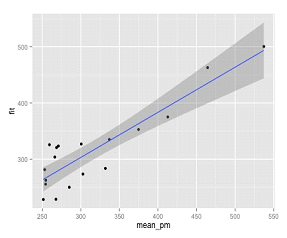
\includegraphics[width=0.6\textwidth]{Figure2-6}
       \caption{Fitted values of a linear regression for outliers in 2015.}
\end{figure}

There was only one meteorological variable is significant, that is mean visibility measured in miles. This variable was kind intuitively reasonable, however, maybe too directly dominant the relationship. So I refitted the model without this variable, it turned out that the mean sea level pressure became significant.

When I could not find a reason with my knowledge to explain the relationship, I decided to see if there is a similar relationship in one particular day. So I took 24  \(PM_{2.5}\) values of January 15 in 2015, did regression on the corresponding meteorological variables within a day. The regression result was shown in Figure 2.7. It turned out that again the sea level pressure was significant with adjusted R-square as highly as 0.77.


 \begin{figure}[!ht]
  \centering
    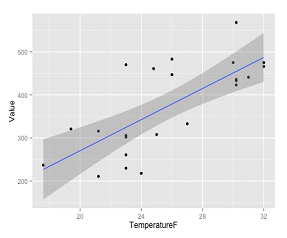
\includegraphics[width=0.6\textwidth]{Figure2-7}
      \caption{Fitted values of a linear regression for \(PM_{2.5}\) values on January 15, 2015.}
\end{figure}

Some ideas about the relationship between \(PM_{2.5}\) and sea level pressure
Beijing is surrounded by mountain ranges that lead to the inversion layer—cold air settles on top of a warmer air mass, trapping the pollutants inside \cite{Hawkins10}. In normal case, air temperature would decrease with altitude. Due to the fact that cold air is denser than warm air, the warmer air near surface is forced to move upward and carries \(PM_{2.5}\) away. In the winter, Beijing’s near surface air cools down much faster than the air high above at night and inversion layer forms (shown in Figure 2.8 below). Colder air sticks near surface and \(PM_{2.5}\) is trapped and starts to accumulation. 


 \begin{figure}[!ht]
  \centering
    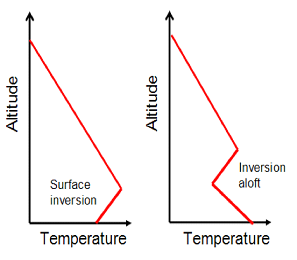
\includegraphics[width=0.6\textwidth]{Figure2-8}
      \caption{Relationship between Temperature and altitude}
\end{figure}

According to ideal gas law: PV=nRT, sea-level pressure is positive related to near surface temperature.  Near surface temperature is minimal when the sea-level pressure is low and cold air would be trapped with \(PM_{2.5}\). In conclusion, sea-level pressure should be negatively related to \(PM_{2.5}\) concentration.





\section{Conclusions and Future Work}

\subsection{Meteorological Regression}

Until now we have not figured out the exact model of \(PM_{2.5}\) concentration on the meteorological factors, because of the limitation of knowledge and data source. If we had more time on the project, we might find ways to deal with these problems and fit a much better model. So far, we only have a sense that \(PM_{2.5}\) concentration does have relationship with meteorological data, and the temperature, wind speed, sea level pressure have negative impacts on the \(PM_{2.5}\) in Beijing, based on a daily average level of one year. However, we have no idea about other variables, such as precipitation, circulation. Thus, in the future, for the regression part, we want to find more explanative predictors for the final model, and explore the specific relationship between \(PM_{2.5}\) concentration and meteorological factors quarterly, based on an hourly level, if data is available. Moreover, try to analyze the results using spatial data, compare the differences of regressions among cities.

\subsection{Outliers:} 

For extreme air pollution events, besides sea level pressure, there must be other factors that will explain part of it, like coal usage during heating time if we can get the data. It’s a cumulative process that eventually result in an outlier. One idea is to find some relationship between one outlier and several days before it, and see if there is a trend or pattern for most of the outliers. 

Lots of missing data--meant for building climate models,
not small-scale, localized projects.

"Self-documenting code", but requires some expert domain
knowledge

Idea is to treat city as a fixed effect
and compute readings by month/day as random effects
with multiple error terms

Makes more sense for grouping dozens of 
messy, missing, spatially-dispersed meteorogical
data with multiple readings--not so useful for
estimating parameters with single samples.

Might be useful for handling "repeated samples" from 
groupings in mornings, afternoon, evening, night. 

More useful for ggplot/organization than for stats
in this project (1 object instead of 5)


\section{Methods and Data Sources}

The United States Department of State measures
air quality data at five locations--the U.S. Embassy in
Beijing, and the Consulates in Chengdu, Guangzhou,
Shanghai, and Shenyang. 

The meteorological data (from the site "Weather Underground") 
contains temperature, dew-point, humidity, sea-level
pressure, visibility, and wind speed.

NOAA Reanalysis dataset--perfect, but way too complicated
to interpret, parse, and group. Simpler datasets
are available.


\begin{thebibliography}{1}

\bibitem{Boren15}
Boren, Zachary D. "China Air Pollution: Beijing Records Its Cleanest Air Ever." 27 Aug. 2015. Accessed from web on Feb. 24, 2016.

\bibitem{Moore14}
Moore, Malcolm. "China's 'airpocalypse' Kills 350,000 to 500,000 Each Year." \textit{The Telegraph}. Telegraph Media Group, 07 Jan. 2014. Accessed from web on Feb. 24, 2016.

\bibitem{Chatani11}
Chatani, Satoru, Tazuko Morikawa, Seiji Nakatsuka, Sou Matsunaga, and Hiroaki Minoura. "Development of a framework for a high-resolution, three-dimensional regional air quality simulation and its application to predicting future air quality over Japan." \textit{Atmospheric Environment} 45, no. 7 (2011): 1383-1393.

\bibitem{Pohjola02}
Pohjola, M. A., A. Kousa, J. Kukkonen, J. Härkönen, A. Karppinen, P. Aarnio, and T. Koskentalo. "The spatial and temporal variation of measured urban PM10 and PM2. 5 in the Helsinki metropolitan area." \textit{Water, Air and Soil Pollution: Focus 2,} no. 5-6 (2002): 189-201.

\bibitem{Tai10}
Tai, Amos PK, Loretta J. Mickley, and Daniel J. Jacob. "Correlations between fine particulate matter (PM 2.5) and meteorological variables in the United States: Implications for the sensitivity of PM 2.5 to climate change." \textit{Atmospheric Environment} 44, no. 32 (2010): 3976-3984.

\bibitem{Hawkins10}
Hawkins, Timothy W., and Lisa A. Holland. "Synoptic and local weather conditions associated with PM2. 5 concentration in Carlisle, Pennsylvania." \textit{Middle States Geographer} 43 (2010): 72-84.

\end{thebibliography}

\end{document}
